
\date{\today}
\title{Webpage Fetch Implementation and Analysis}


\documentclass[12pt]{article}

\usepackage{graphicx}

\author{
  Singhal, Madhur\\
  \texttt{2015CS10235}
  \and
  Chhajwani, Anant\\
  \texttt{2015CS50281}
}

\begin{document}
\maketitle


\section{Introduction}

In this assignment we implemented a multi-threaded web browser. We used \textbf{multilevel multi-threading} with each domain having it's own thread and each socket connection having it's own sub-thread.
\paragraph{}
Sending multiple requests for content in parallel reduces the total page load time substantially. Establishing a socket connection has some overhead so taking the stated approach to the extreme and having a socket for every request in parallel is inefficient. Thus there needs to be a compromise to select the appropiate number of sockets per domain and the number of requests handled by any socket. In this assignment we present a basic empirical analysis.
\section{Description}
The \textbf{HAR (HTTP Archive Format)} files generated by a normal web browser record all the requests made by the browser. We extract all the requests from a given HAR file and put them into a format satisfying the HTTP conventions. After this we can open TCP sockets to the hosts and send them the generated requests. 
\paragraph{}
We accept two parameters, the number of sockets to open for each domain and the number of objects to download over each socket. We use a sliding window algorithm for each domain so that new threads are created as soon as old ones reach their ibject limit. Our analysis consists of varying the parameters and observing the effect in terms of the total download time.
\section{Comparison of Page Load time}

We used the `indianexpress.com' page to compare page load times for. We varied the parameter values and compared page load times for different combinations.

%\begin{center}
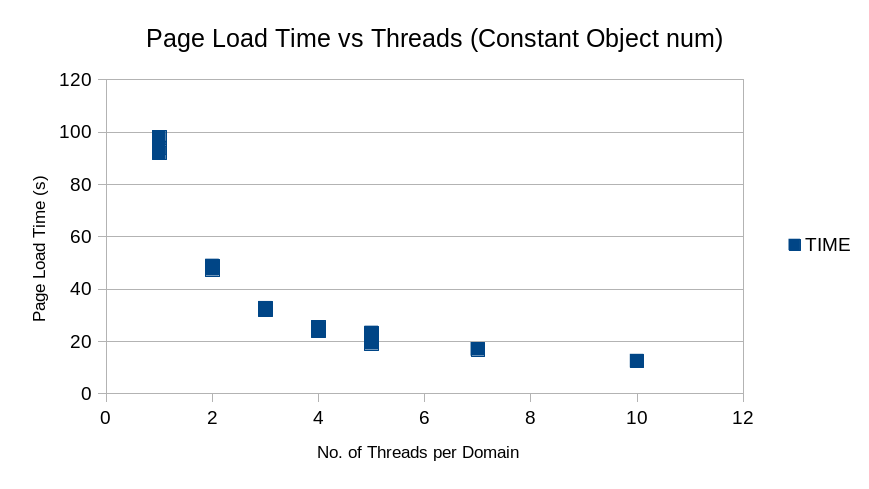
\includegraphics[scale=1]{q4_1.png}
%\end{center}

%\begin{center}
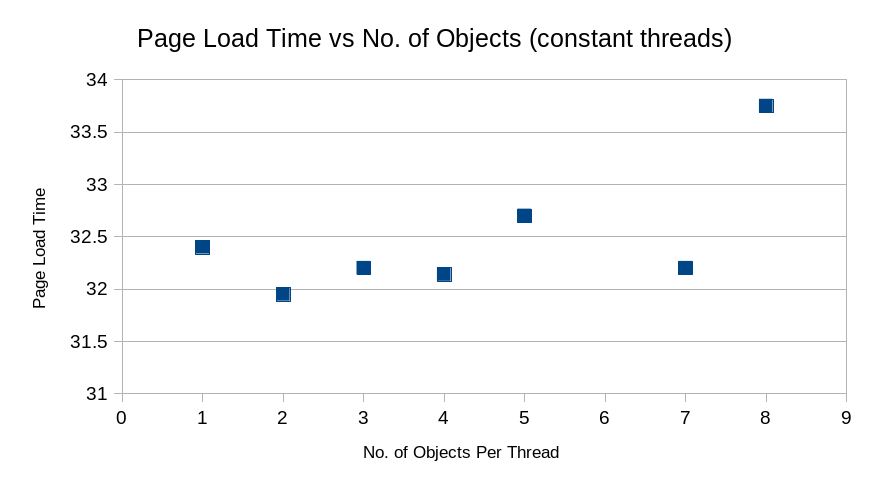
\includegraphics[scale=1]{q4_2.png}
%\end{center}

For this particular site we observe that the page load time falls dramatically as we increase the number of threads while changing the number of objects per thread barely affects the load time.  This is reasonable since this website contains a lot of images which comprise the bulk of the time invested and increasing the number of threads makes the image downloads happen in parallel. Increasing the number of objects per thread just reduces the overhead so it does not affect the page load time dramatically since the overhead involved is small in comparision to the size of the images.\\
 The best choice of parameter values in this case was actually found to be  70 threads with 1 download per thread (2.01 seconds). This is not shown on the graph since the graph would be very hard to read otherwise. The reason we observed this is likely because this experiment was done on a very high bandwidth machine (1 Gbps) and so in the optimal case there is just one thread for each download to be done.\\
This was slightly lower than the browser page load time of 3.43 seconds. A big factor  is the fact that in our program all HTTPS resources are ignored but the browser processes them too. Also the browser may have some set of prebuilt parameters while we optimize for the best one by trying  many combinations.
\section{Estimating Optimal Parameters}
To estimate the optimal parameters we need information about the distribution of sizes of the components of the website and information about our network connection to the server. More specifically in the former area we would like to know whether the website consists of a large number of small components, in which case we want many of those to be downloaded over the same socket, or  a small number of big files, in which case we want a number of threads fetching those files in parallel. In the latter category we would like information about the banwidth of our connection to the server, the latency and maybe even the load on the server.\\
\textbf{Possible Modifications} -
\begin{enumerate}
\item The HTML standard can be modified to require that each webpage include a histogram of the sizes of the requests needed to be made to load that particular webpage.
\item The HTTP standard can be modified to require that servers also specify how much load they are under and how many more socket connections they can support at any particular moment so that browsers may choose to not open more sockets.
\item The Application Layer Protocols can be modified by merging simple network monitoring tools like a ping test and a bandwidth test so that each connection knows it's bandwidth and latency.
\item The Link and Network Layers can be modified to require that information like the number of hops and error rate be visible to higher layers so they may decide to open more sockets if the error rate is low and less sockets if the error rate is high.
\end{enumerate}

\end{document}